\chapter{Visualisasi}
\begin{mybox}{Anggota Kelompok}
\begin{enumerate}
    \itemsep0em
    \item Citra Putri Saragih (25/574147/PPA/07239)
    \item Ade Dwi Putra (25/574144/PPA/07237)
\end{enumerate}
\end{mybox}

\section{Skenario dan Pengguna Dashboard}

Visualisasi dibangun di atas data mart perjalanan bus antarkota yang telah
dihasilkan pada Bab 1. Pengguna dashboard terdiri atas VP of Operations, VP
Commercial and Revenue Management, serta Head of Customer Loyalty. Bagian
operasional membutuhkan informasi keterlambatan, pelanggaran SLA, dan kegagalan
koneksi. Bagian komersial menggunakan informasi kerugian akibat gangguan
perjalanan, sedangkan bagian loyalitas memantau pola transaksi dan penggunaan
poin penumpang.

Data yang ditampilkan bersifat sintetis. Hasil visualisasi digunakan untuk
menunjukkan kemampuan data mart dalam menjawab kebutuhan analitik dan tidak
dimaksudkan untuk menggambarkan kondisi operator bus tertentu.

\section{Tools Visualisasi}

\subsection{Tableau}

Tableau digunakan untuk membentuk relationship antara fact table dan dimension
table, membuat calculated field, serta menyusun dashboard interaktif. Tiga
dashboard dibuat dalam satu workbook untuk memisahkan analisis operasional,
penjualan tiket, dan transaksi loyalitas.

\subsection{Python-based Tools}

Tool kedua menggunakan pandas, Plotly, dan Streamlit. Pandas digunakan untuk
membaca serta menggabungkan keluaran data mart, Plotly untuk membentuk grafik,
dan Streamlit sebagai antarmuka dashboard. Implementasinya ditempatkan dalam satu
berkas \texttt{dashboard.py}.

Kedua tools membaca berkas CSV pada direktori \texttt{data-mart/output}. Tidak ada
dataset baru yang dibangkitkan pada tahap visualisasi. Workbook Tableau disimpan
dalam format \texttt{.twbx} agar worksheet, relationship, dan sumber data berada
dalam satu berkas.

\section{Perancangan Dashboard}

Dashboard Tableau dibagi menjadi tiga bagian berdasarkan proses bisnis:

\begin{enumerate}[label=\alph*., leftmargin=*]
    \item \textbf{Kinerja Operasional dan Dampak Finansial}, untuk menganalisis
    arrival delay, status SLA, missed connection, dan revenue leakage;
    \item \textbf{Loyalitas dan Perilaku Penumpang}, untuk membandingkan jumlah
    tiket, pendapatan rata-rata, dan penggunaan poin pada setiap loyalty tier; dan
    \item \textbf{Aktivitas Transaksi Loyalitas}, untuk melihat jumlah transaksi,
    mutasi poin, serta perubahan aktivitas loyalitas setiap bulan.
\end{enumerate}

Pembagian tersebut mengikuti tiga fact table pada data mart sehingga measure
dengan grain berbeda tidak digabungkan secara langsung dalam satu tabel datar.

\subsection{Definisi Metrik}

\begin{itemize}
    \item \textit{Missed connection rate} adalah jumlah
    \texttt{missed\_connection\_count} dibagi jumlah itinerary leg yang diamati.
    \item Status \textit{SLA breach} diberikan pada perjalanan dengan
    \texttt{arrival\_delay\_minutes} lebih dari 60 menit.
    \item \textit{Revenue leakage} merupakan jumlah \texttt{rebooking\_cost},
    \texttt{refund\_amount}, dan \texttt{compensation\_amount} pada klaim yang
    disetujui selama peak season.
    \item Aktivitas poin dibedakan menjadi \texttt{EARN} sebagai poin masuk dan
    \texttt{REDEEM} sebagai poin keluar.
\end{itemize}

\section{Implementasi Python-based Tools}

Program membaca tiga fact table dan dimension table yang relevan. Penggabungan
dilakukan melalui surrogate key yang telah dibentuk oleh ETL, kemudian hasil
agregasi disiapkan untuk ditampilkan melalui antarmuka Streamlit.

Dashboard menyediakan lima kelompok analisis yang mengikuti business questions,
yaitu missed connection, delay dan SLA, revenue leakage, perbandingan loyalty
tier, serta repeat booking. Pada analisis armada, data diringkas menjadi satu baris
per \texttt{trip\_id} terlebih dahulu karena grain fact perjalanan berada pada
tingkat penumpang-leg. Dengan cara ini, satu keterlambatan bus tidak dihitung
berulang untuk seluruh penumpang dalam perjalanan yang sama.

Tabel hasil agregasi disediakan bersama grafik agar angkanya dapat dibandingkan
dengan query verifikasi pada Bab 1.6. Analisis repeat booking diperlakukan sebagai
asosiasi, bukan hubungan sebab-akibat, karena data tidak mengendalikan seluruh
faktor yang dapat memengaruhi perilaku pemesanan penumpang.

\subsection{Hasil Dashboard Python}

\begin{figure}[htbp]
    \centering
    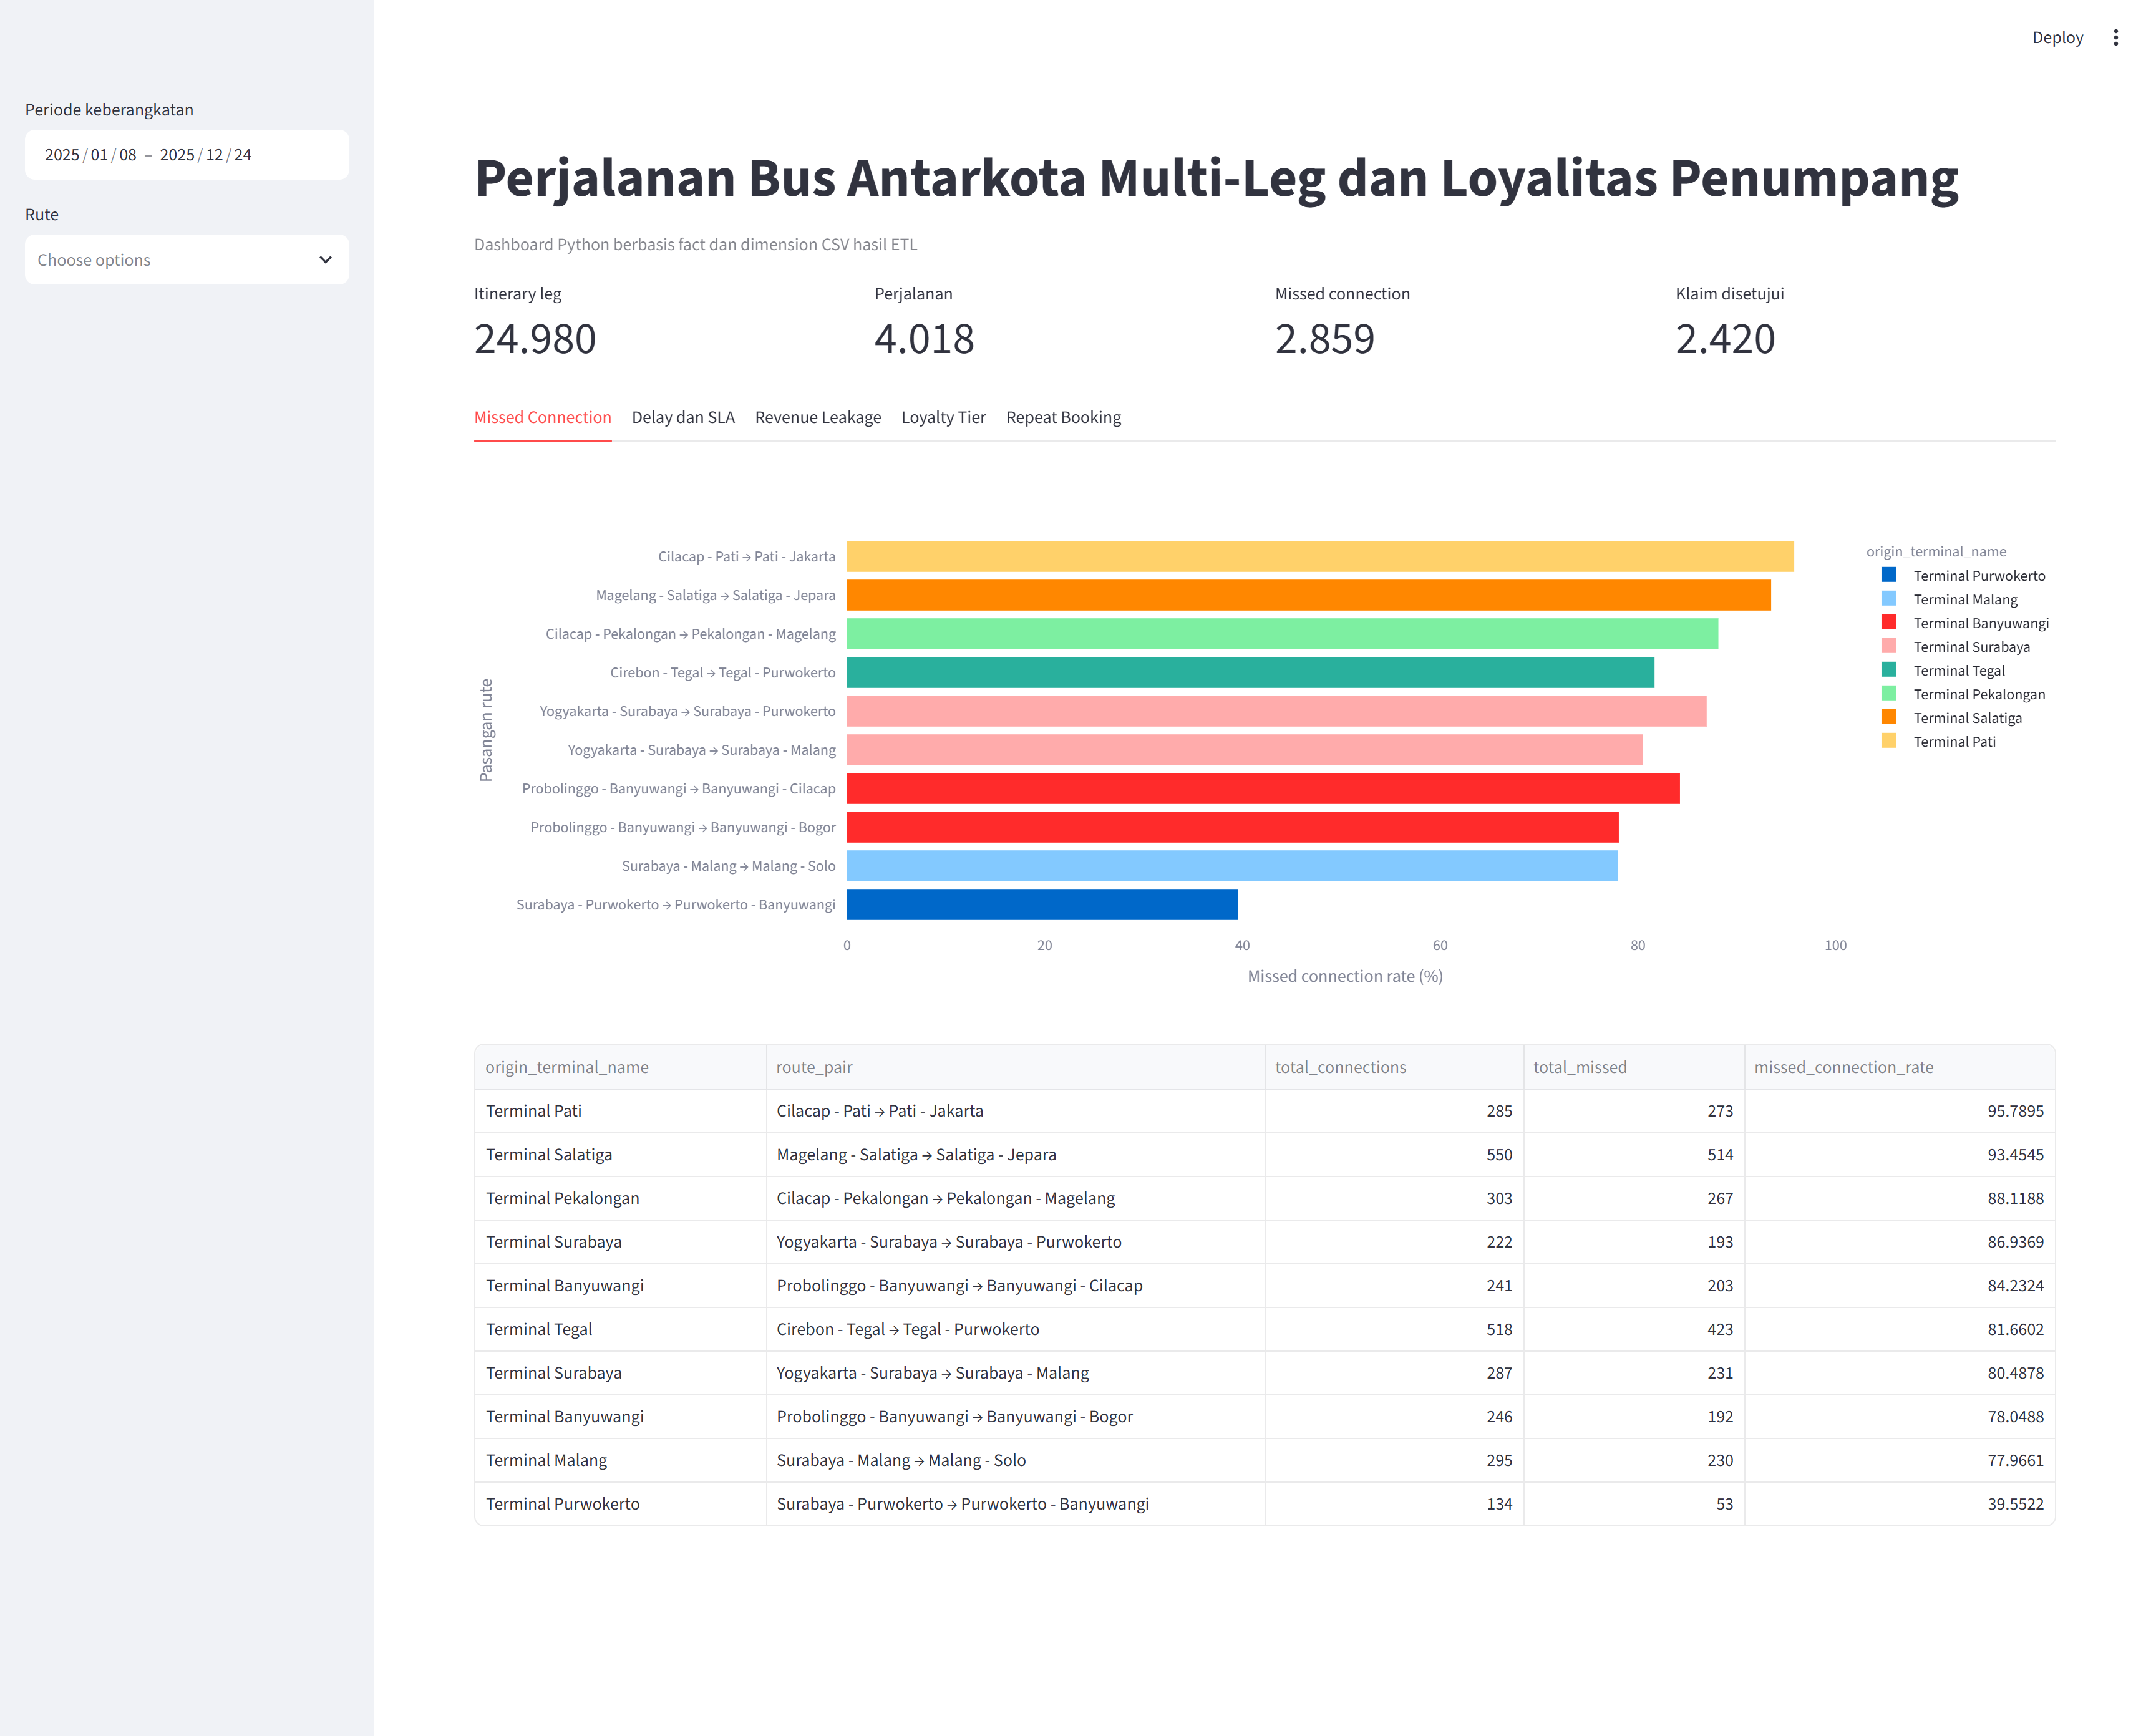
\includegraphics[width=0.9\textwidth]{figures/python-missed-connection.png}
    \caption{Analisis missed connection menggunakan Python}
    \label{fig:python-missed-connection}
\end{figure}

Gambar \ref{fig:python-missed-connection} menunjukkan pasangan Cilacap--Pati dan
Pati--Jakarta sebagai koneksi dengan missed connection rate tertinggi, yaitu
95,79 persen dari 285 koneksi. Urutan hasilnya sama dengan query pertama pada
Bab 1.6.

\begin{figure}[htbp]
    \centering
    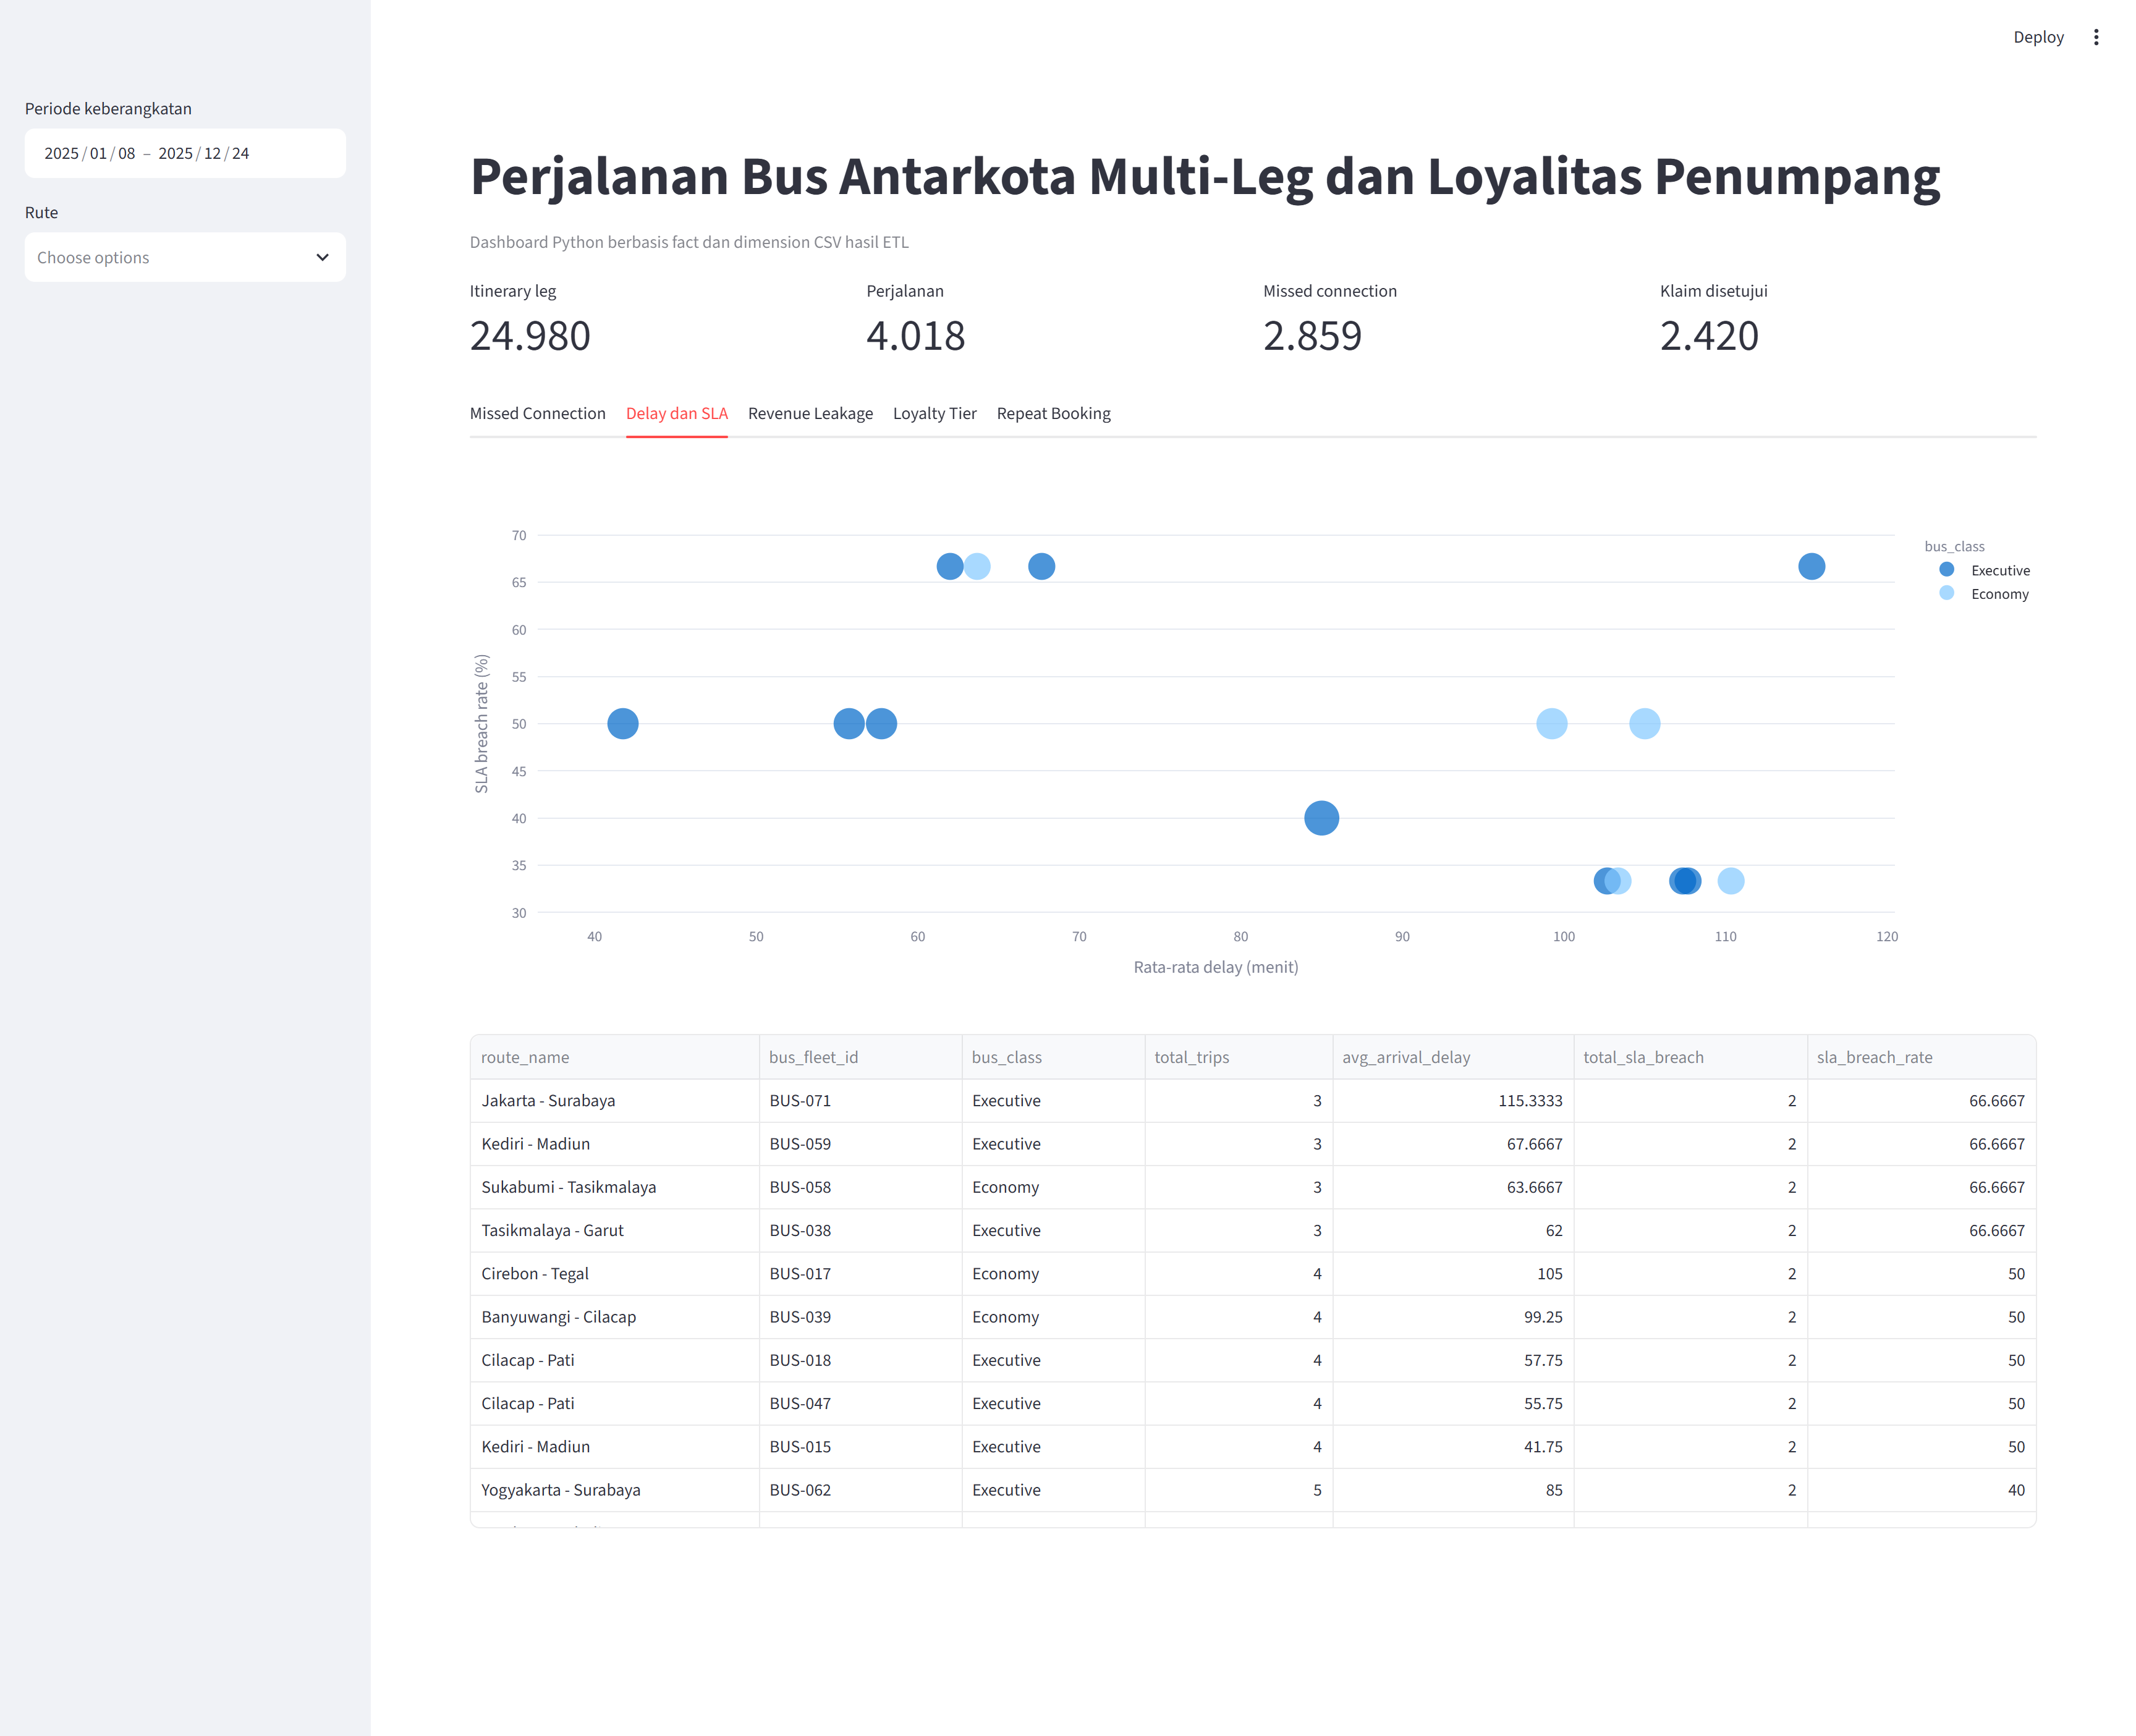
\includegraphics[width=0.9\textwidth]{figures/python-delay-sla.png}
    \caption{Analisis arrival delay dan SLA menggunakan Python}
    \label{fig:python-delay-sla}
\end{figure}

Visual delay dan SLA pada Gambar \ref{fig:python-delay-sla} menggunakan satu
observasi per trip. Kombinasi Jakarta--Surabaya dan BUS-071 memiliki rata-rata
delay 115,33 menit dengan SLA breach rate 66,67 persen dari tiga perjalanan.

\begin{figure}[htbp]
    \centering
    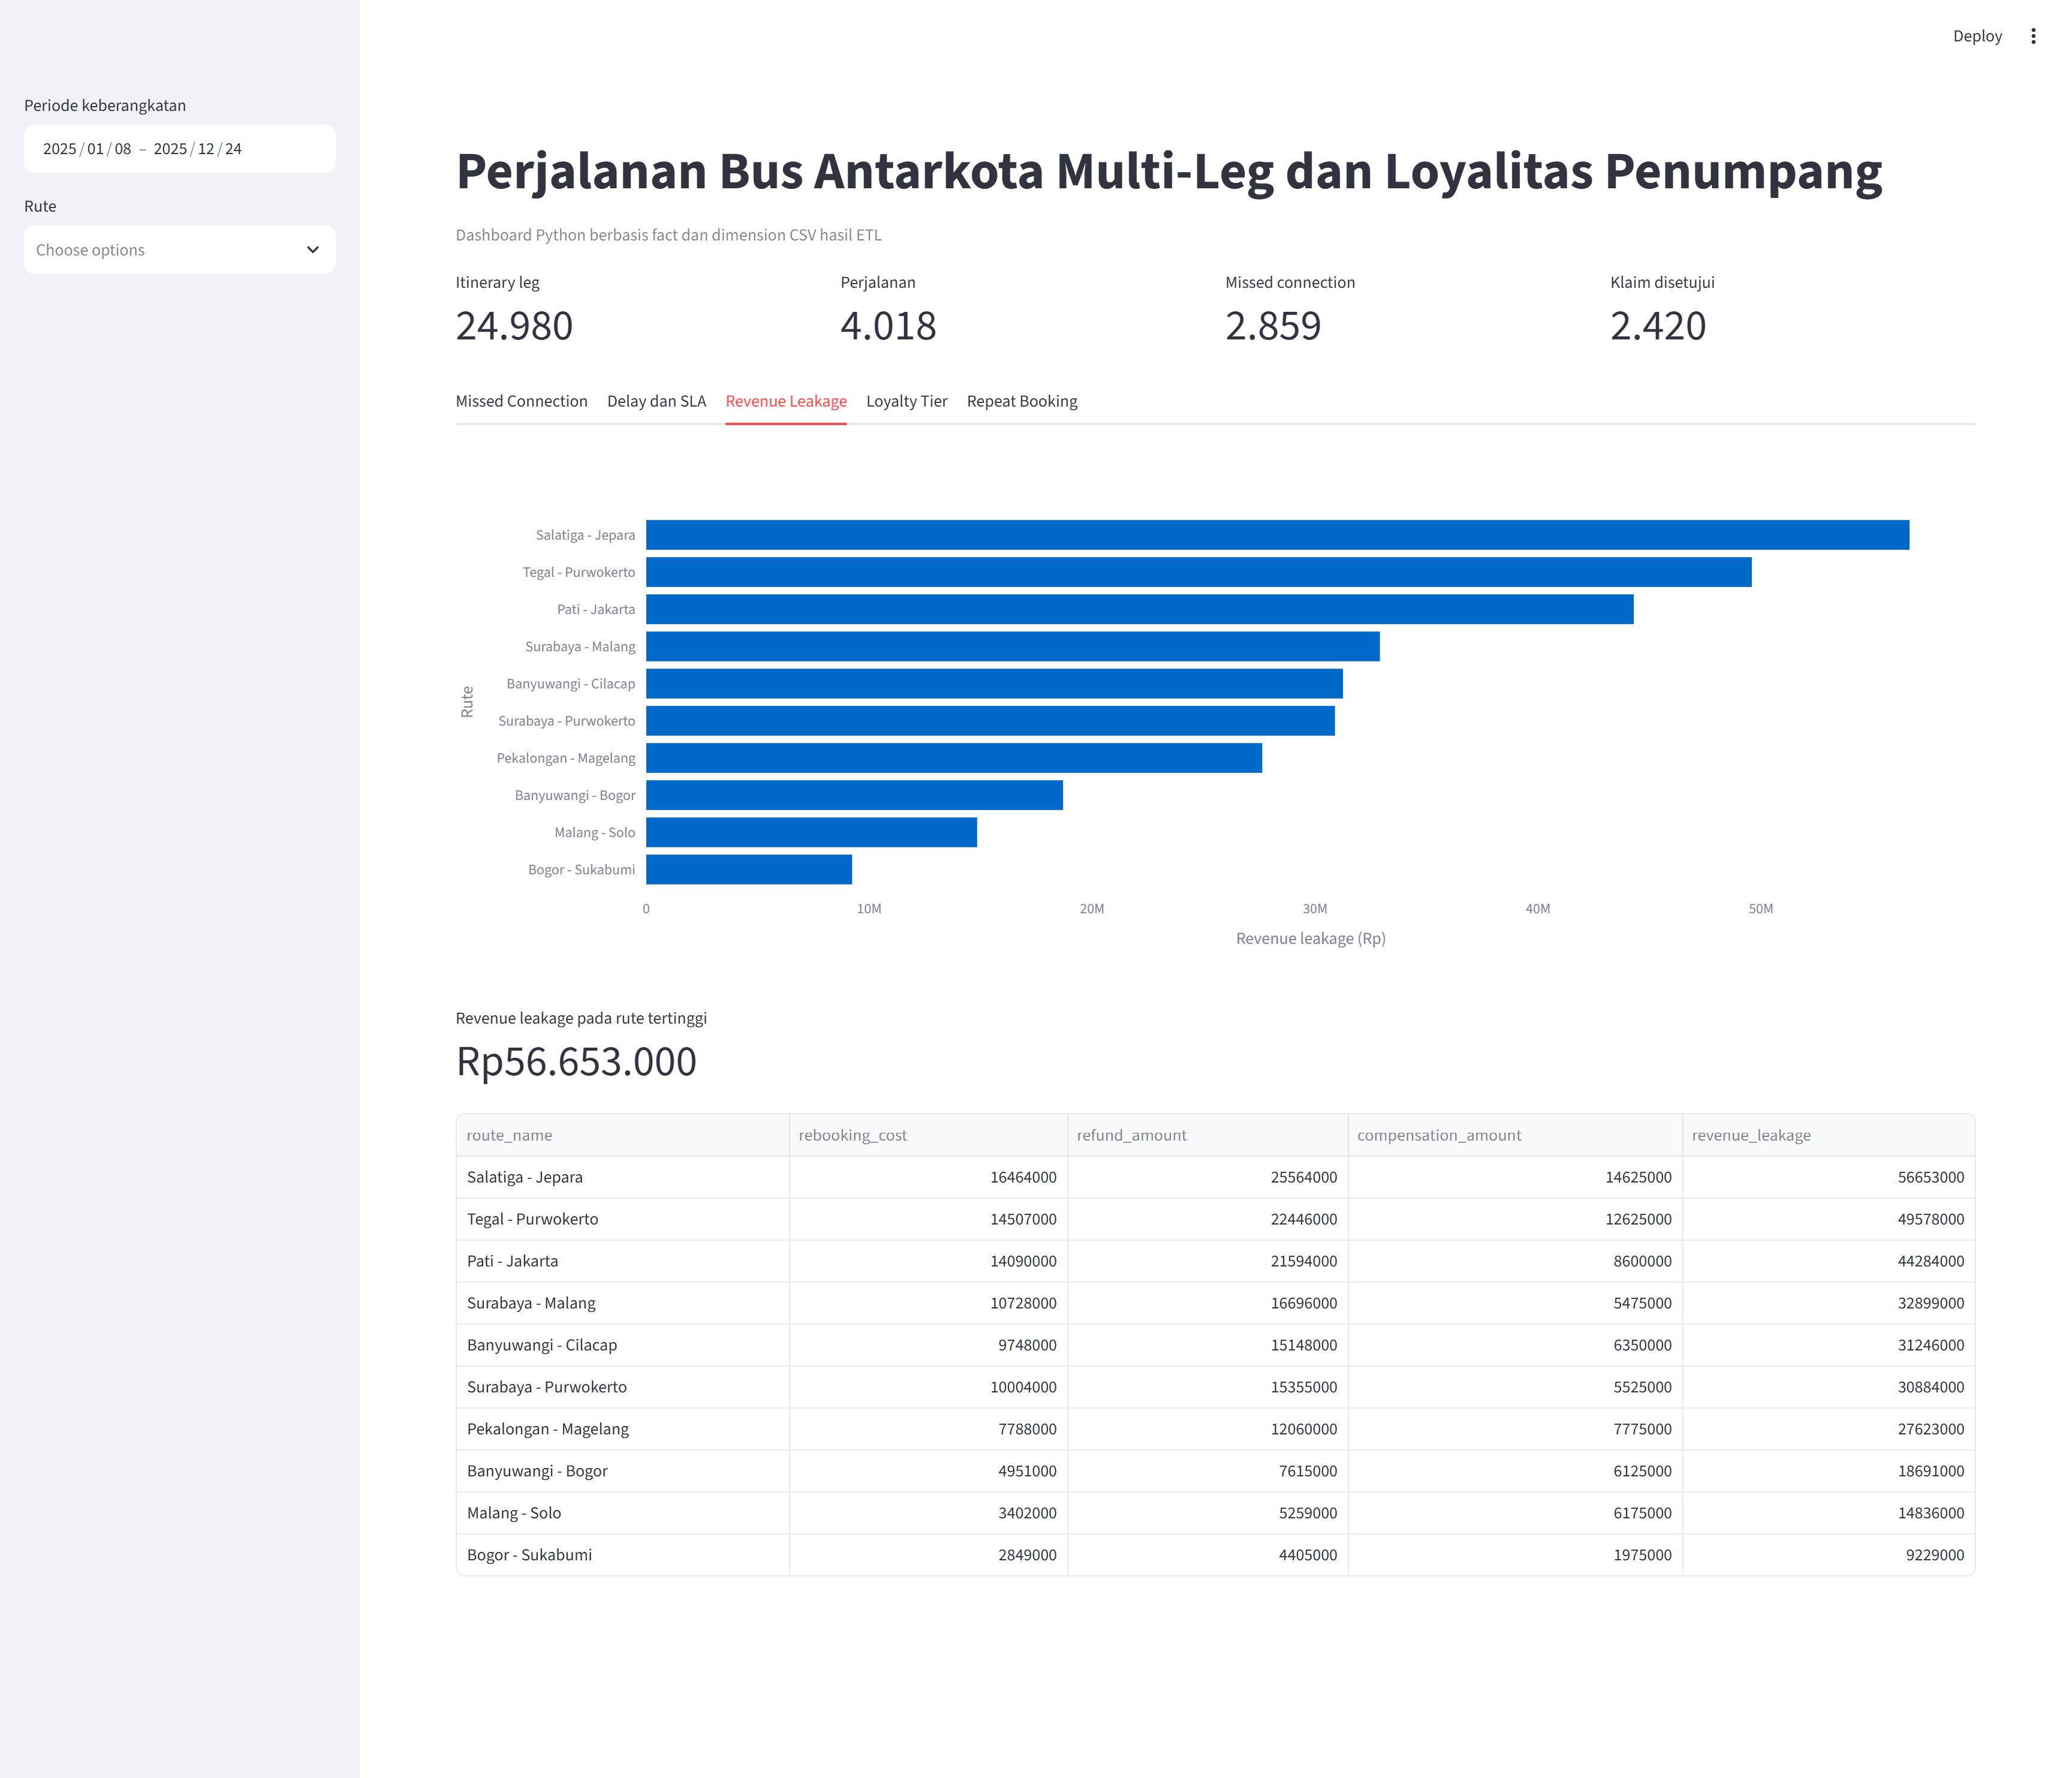
\includegraphics[width=0.9\textwidth]{figures/python-revenue-leakage.png}
    \caption{Analisis revenue leakage menggunakan Python}
    \label{fig:python-revenue-leakage}
\end{figure}

Gambar \ref{fig:python-revenue-leakage} memperlihatkan rute Salatiga--Jepara
sebagai rute dengan revenue leakage tertinggi pada peak season, yaitu
Rp56.653.000. Nilai tersebut berasal dari refund, biaya rebooking, dan kompensasi
pada klaim yang disetujui.

\begin{figure}[htbp]
    \centering
    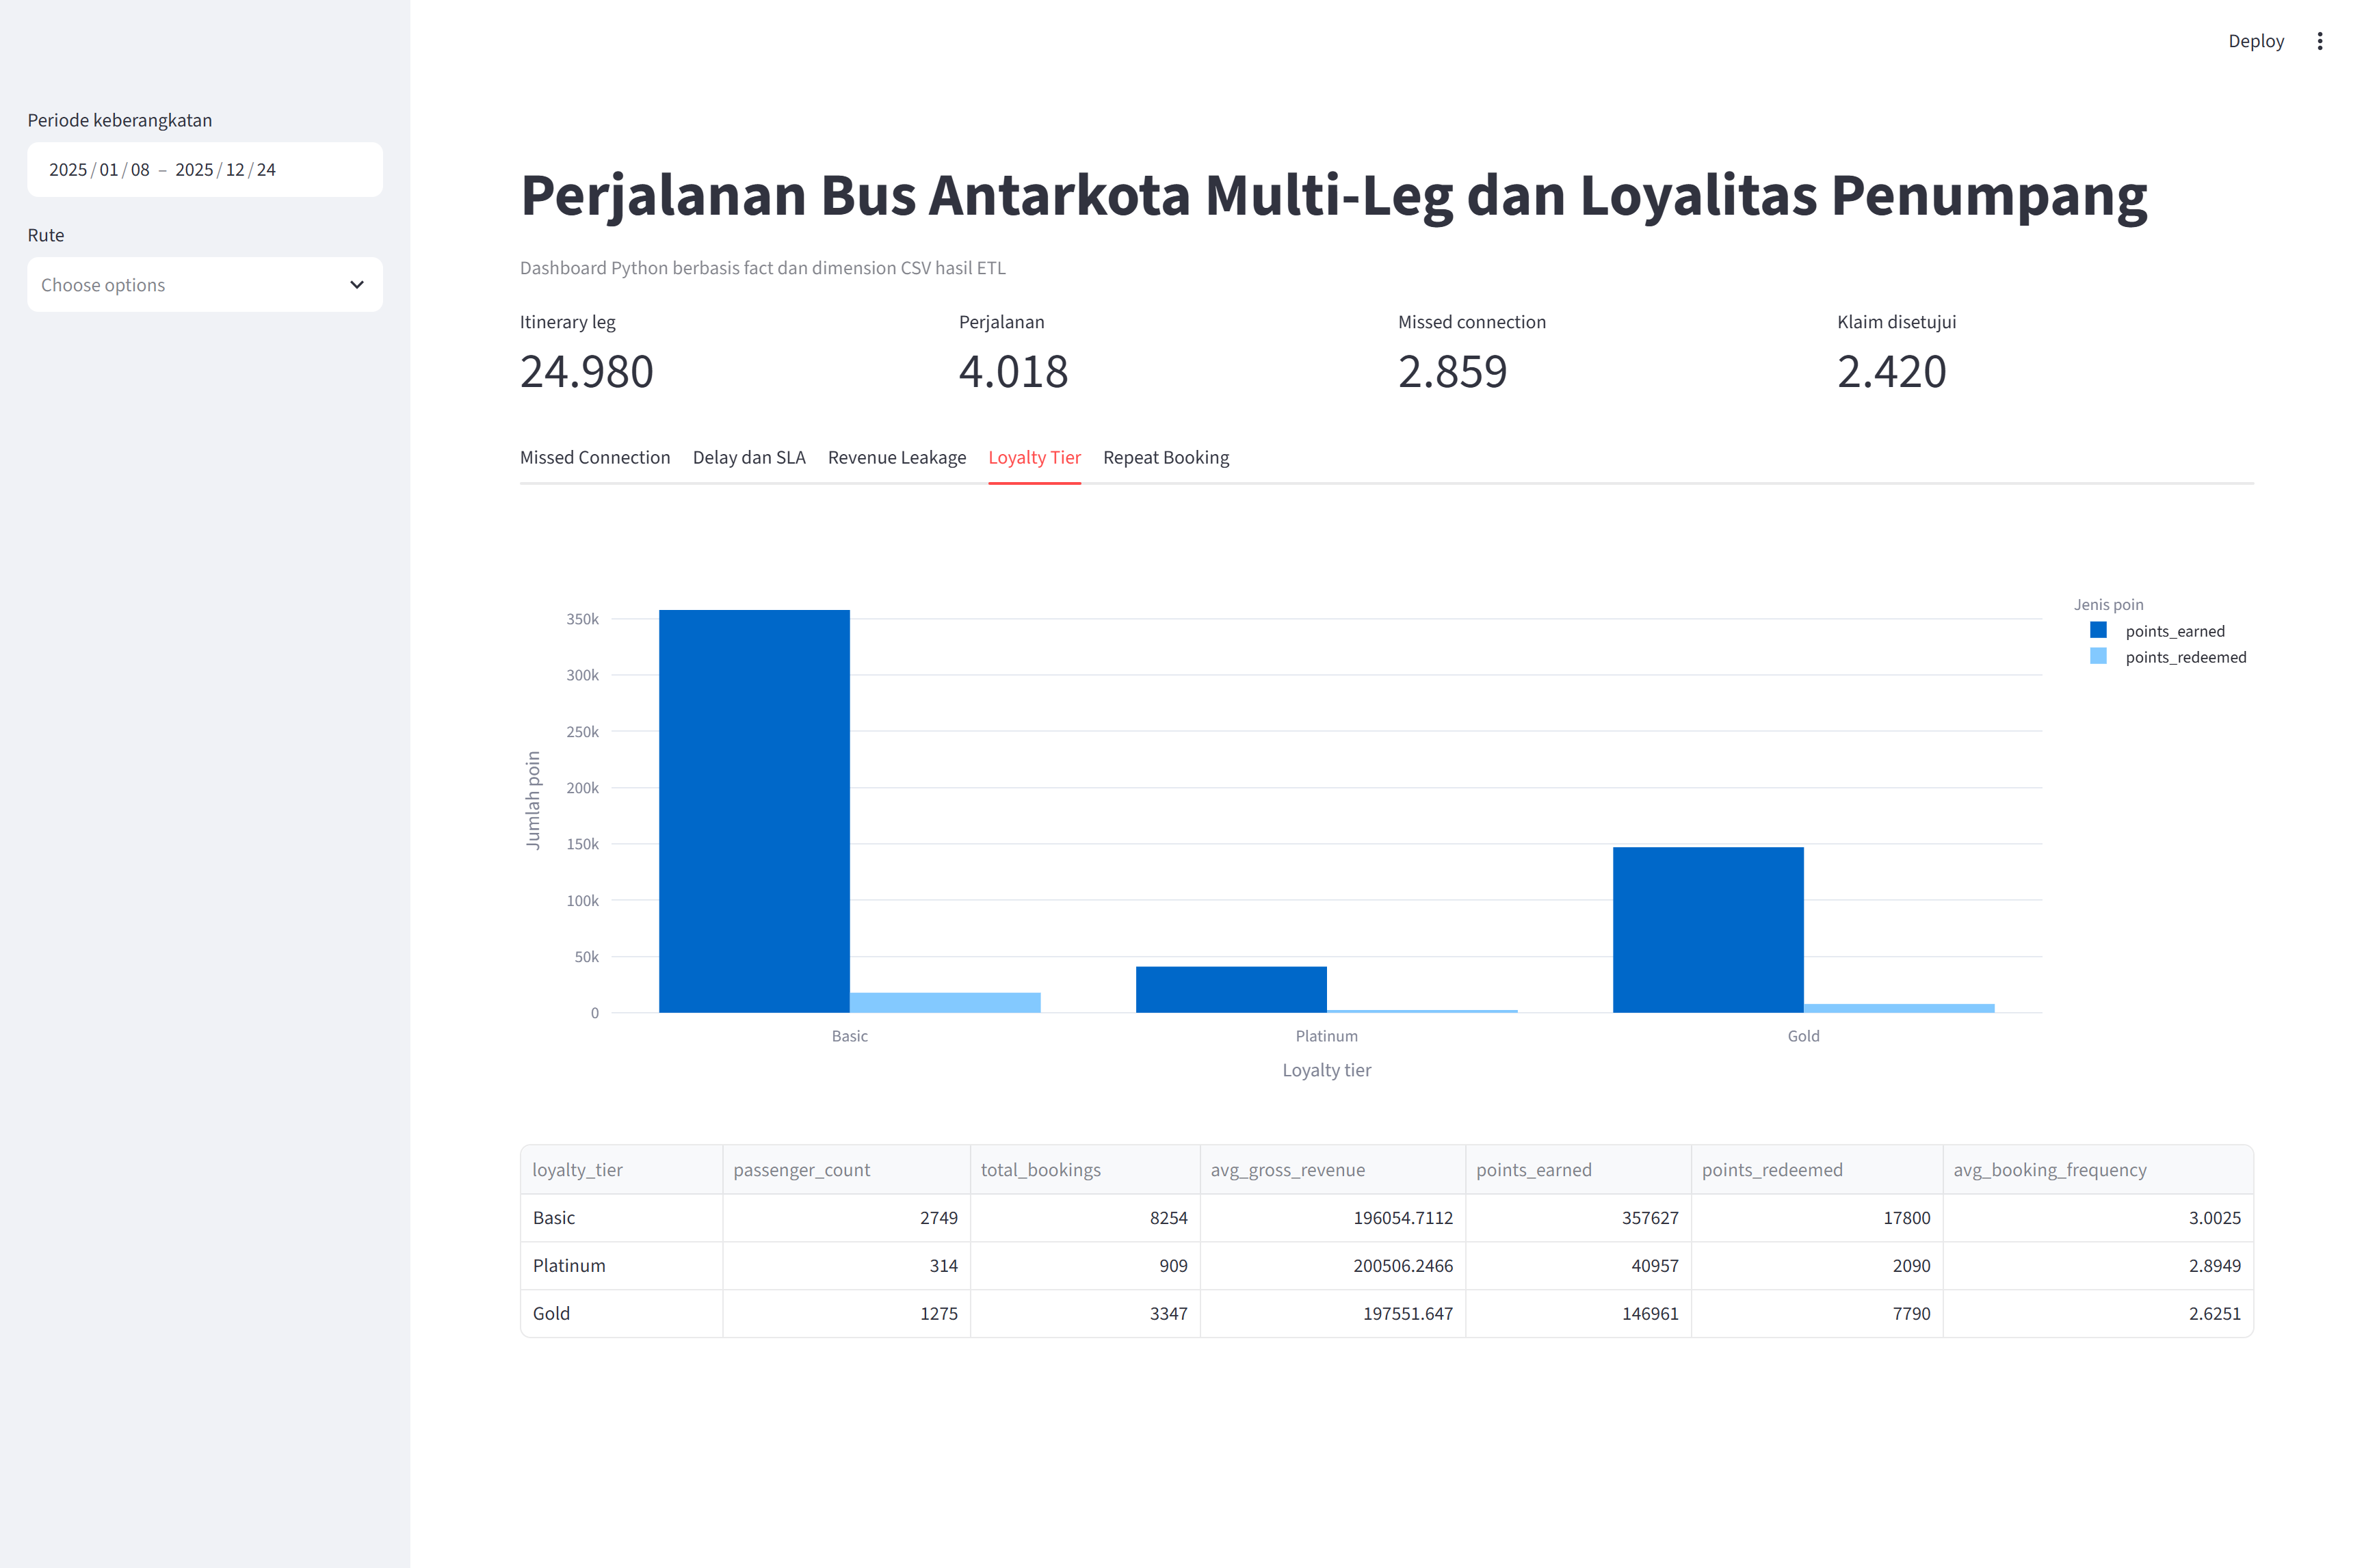
\includegraphics[width=0.9\textwidth]{figures/python-loyalty-tier.png}
    \caption{Perbandingan aktivitas berdasarkan loyalty tier menggunakan Python}
    \label{fig:python-loyalty-tier}
\end{figure}

Perbandingan pada Gambar \ref{fig:python-loyalty-tier} menunjukkan bahwa Basic
memiliki jumlah booking dan penumpang terbesar, sementara pendapatan rata-rata
tertinggi terdapat pada Platinum. Grafik poin juga memperlihatkan bahwa perolehan
poin lebih dominan daripada penukarannya pada seluruh tier.

\begin{figure}[htbp]
    \centering
    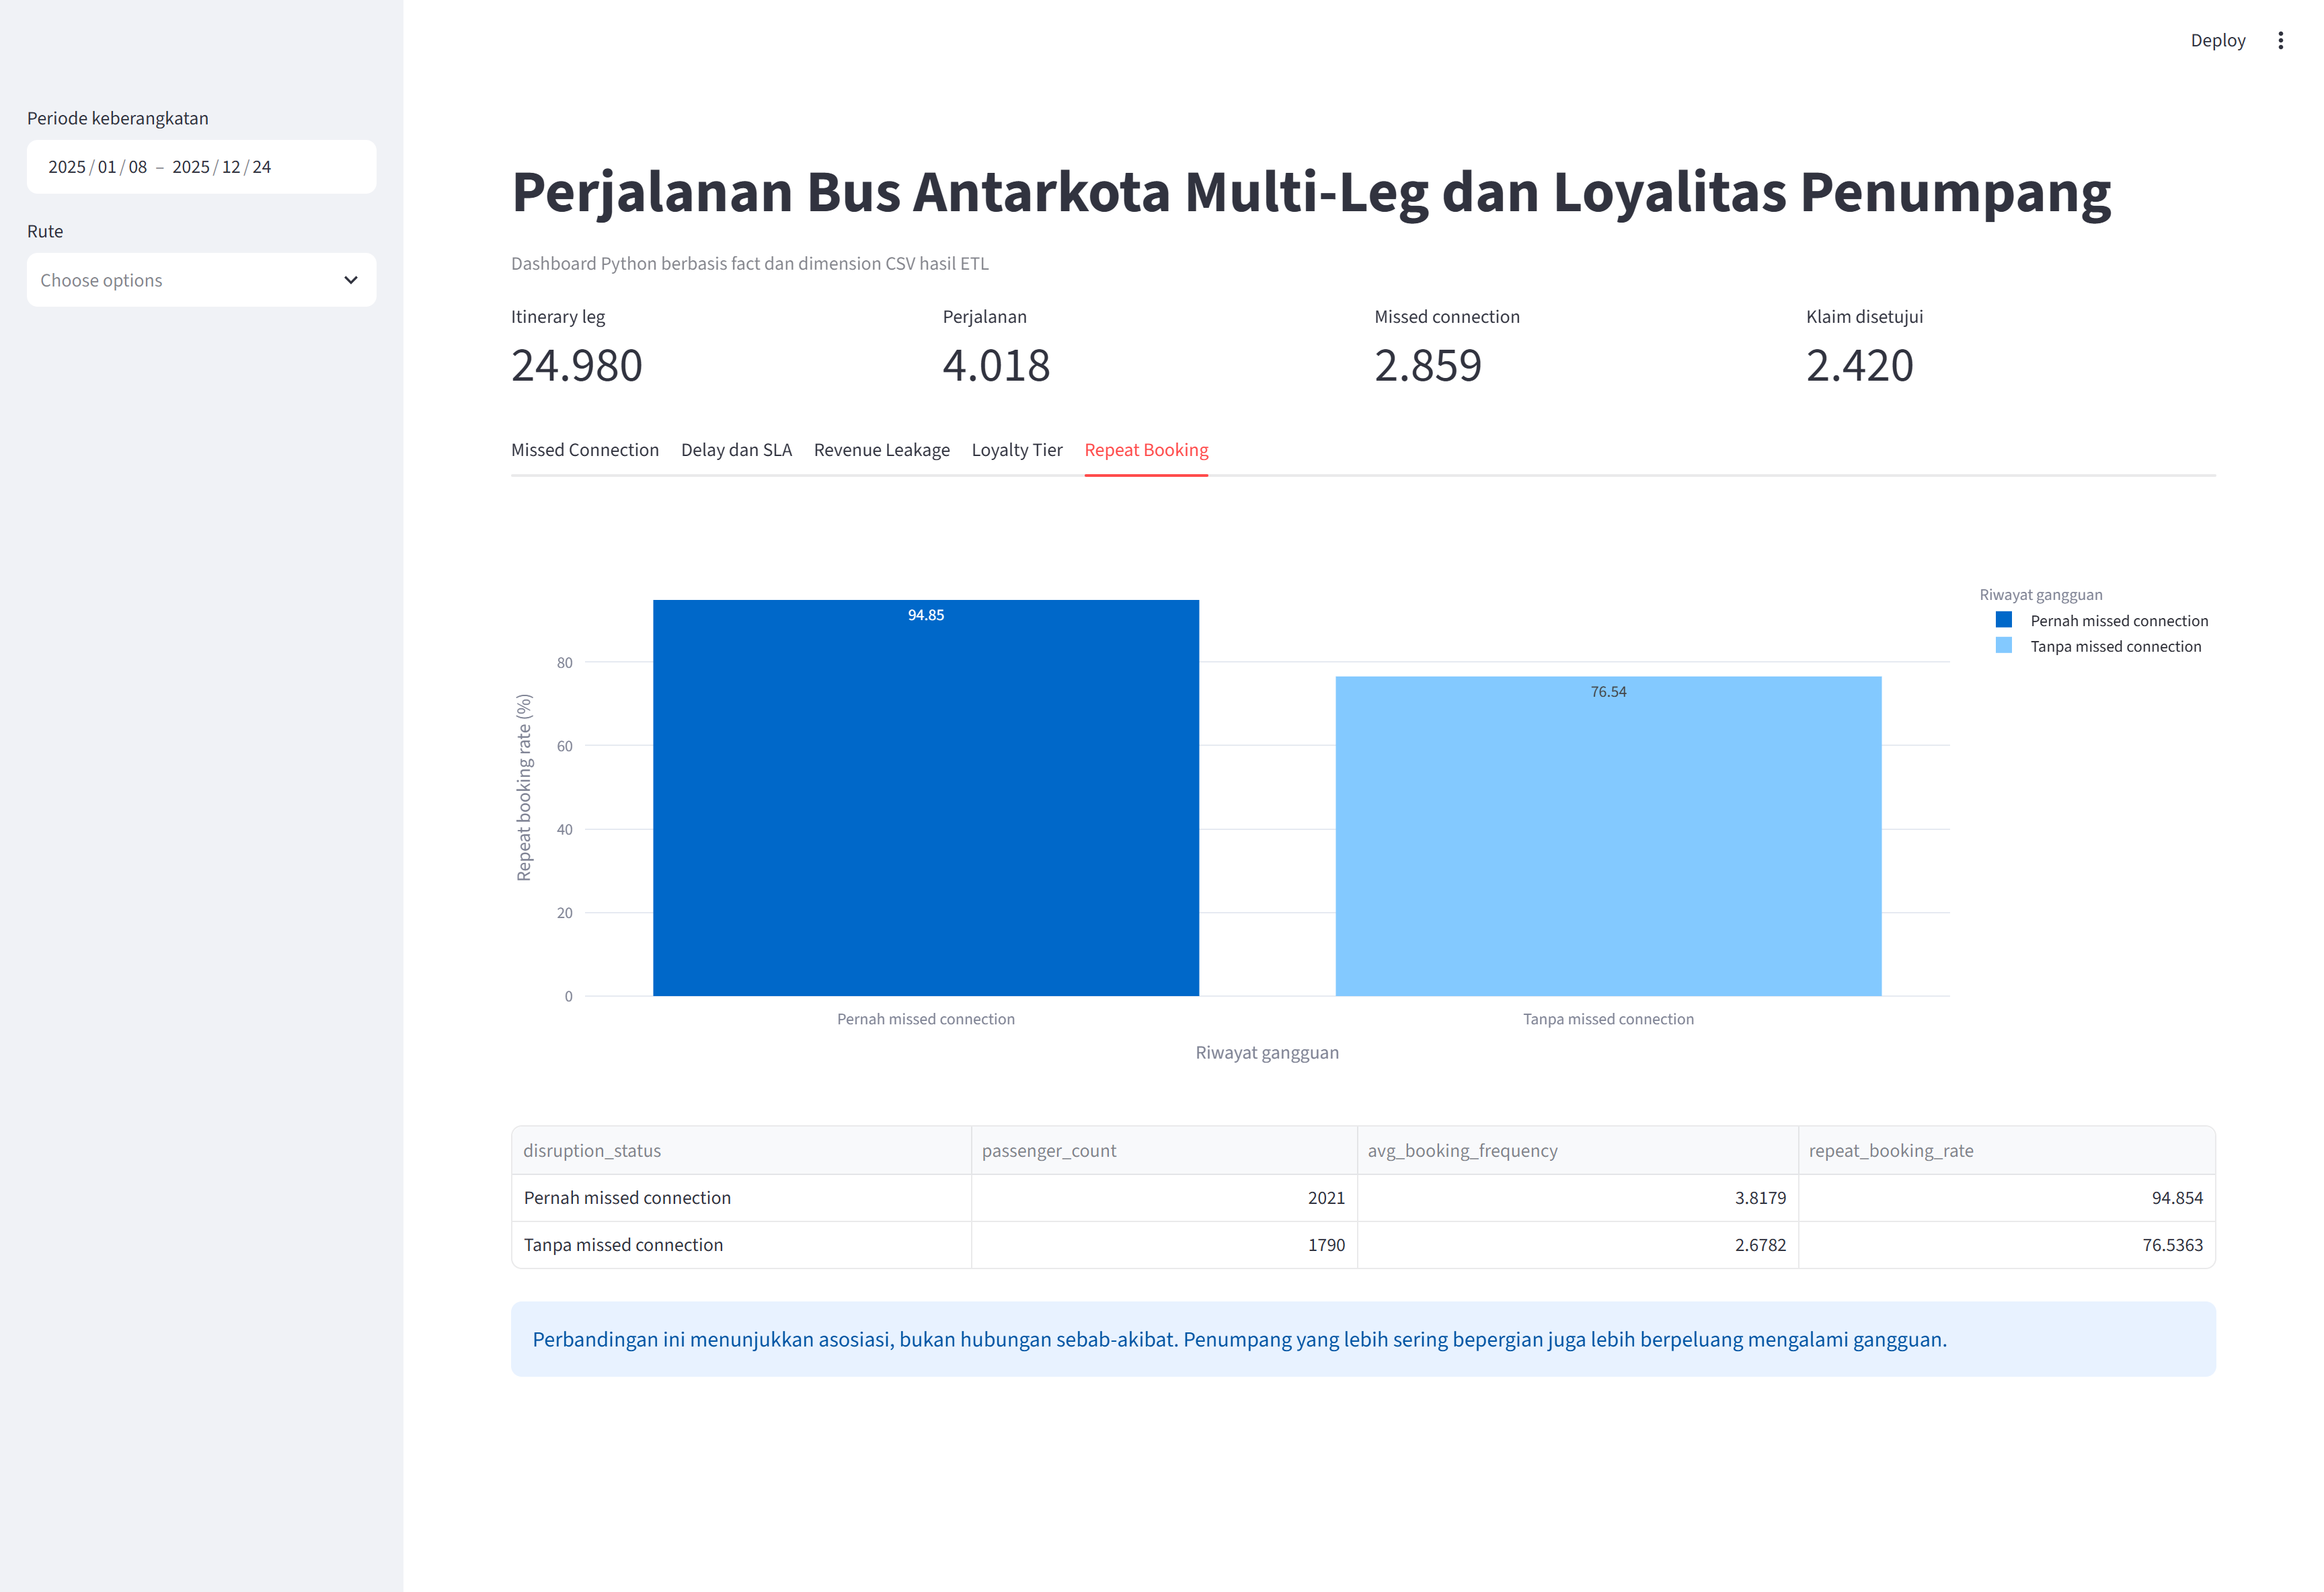
\includegraphics[width=0.9\textwidth]{figures/python-repeat-booking.png}
    \caption{Perbandingan repeat booking berdasarkan riwayat gangguan}
    \label{fig:python-repeat-booking}
\end{figure}

Gambar \ref{fig:python-repeat-booking} memperlihatkan repeat booking rate sebesar
94,85 persen pada penumpang yang pernah mengalami missed connection dan 76,54
persen pada kelompok tanpa missed connection. Hasil ini menunjukkan asosiasi pada
data sintetis, bukan hubungan sebab-akibat.

\section{Hasil Implementasi Tableau}

\subsection{Konfigurasi Data Source}

Tiga data source dibentuk dengan menempatkan satu fact table sebagai tabel pusat.
Data source operasional menggunakan
\texttt{fct\_passenger\_itinerary\_leg}, data source penjualan menggunakan
\texttt{fct\_ticket\_sales}, dan data source transaksi loyalitas menggunakan
\texttt{fct\_loyalty\_transaction}. Dimension table dihubungkan menggunakan
relationship berdasarkan surrogate key berakhiran \texttt{\_sk}.

Pemisahan tersebut mempertahankan grain masing-masing fact table dan mengurangi
risiko fan-out. Dimension table yang digunakan bersama, seperti
\texttt{dim\_passenger}, \texttt{dim\_date}, dan \texttt{dim\_route}, tetap
berperan sebagai conformed dimensions. Calculated field yang digunakan meliputi
\texttt{SLA Status}, \texttt{Connection Leg}, \texttt{Missed Connection Rate},
dan \texttt{Revenue Leakage}.

\subsection{Dashboard Kinerja Operasional dan Dampak Finansial}

\begin{figure}[htbp]
    \centering
    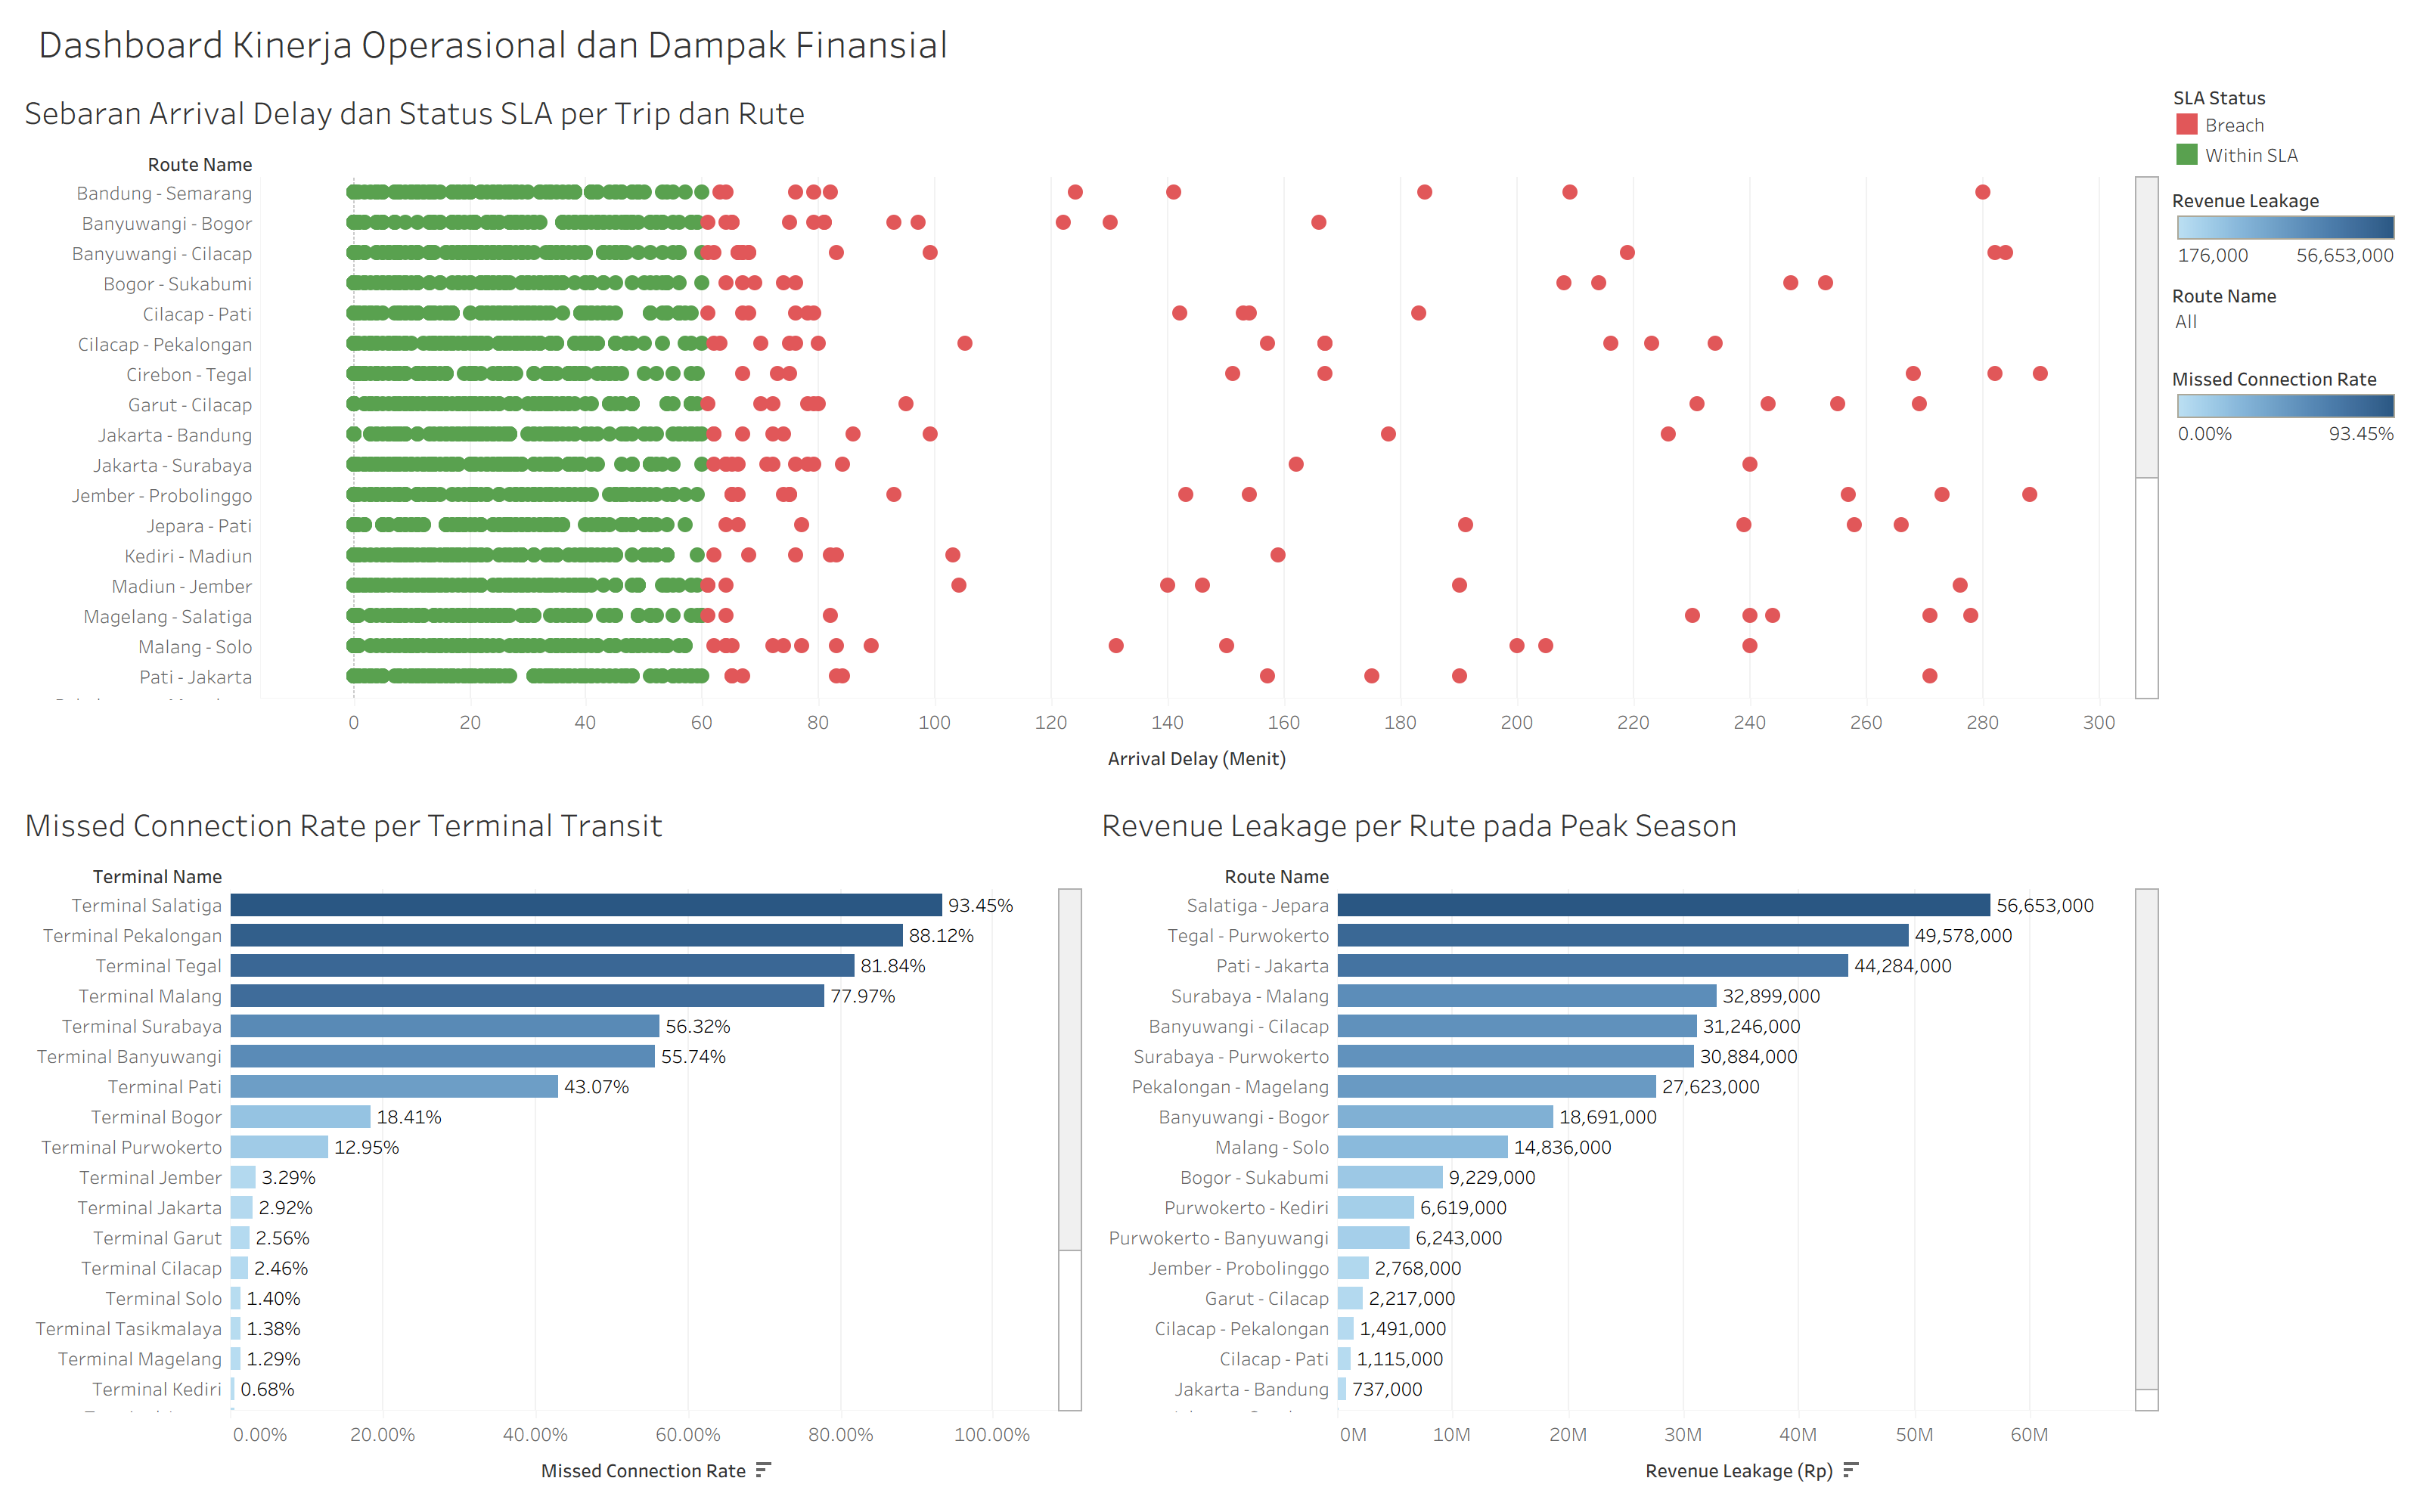
\includegraphics[width=\textwidth]{figures/dashboard-operasional.png}
    \caption{Dashboard kinerja operasional dan dampak finansial}
    \label{fig:dashboard-operasional}
\end{figure}

Gambar \ref{fig:dashboard-operasional} memperlihatkan sebaran arrival delay pada
setiap rute. Titik merah menunjukkan keterlambatan di atas batas SLA 60 menit,
sedangkan titik hijau masih berada dalam SLA. Beberapa perjalanan memiliki delay
lebih dari 200 menit sehingga terlihat sebagai outlier operasional.

Terminal Salatiga memiliki missed connection rate tertinggi, yaitu 93,45 persen,
disusul Terminal Pekalongan sebesar 88,12 persen dan Terminal Tegal sebesar 81,84
persen. Pada peak season, rute Salatiga--Jepara mencatat revenue leakage terbesar
sebesar Rp56.653.000, kemudian Tegal--Purwokerto sebesar Rp49.578.000 dan
Pati--Jakarta sebesar Rp44.284.000. Filter rute dapat digunakan untuk mempersempit
analisis ke rute tertentu.

\subsection{Dashboard Loyalitas dan Perilaku Penumpang}

\begin{figure}[htbp]
    \centering
    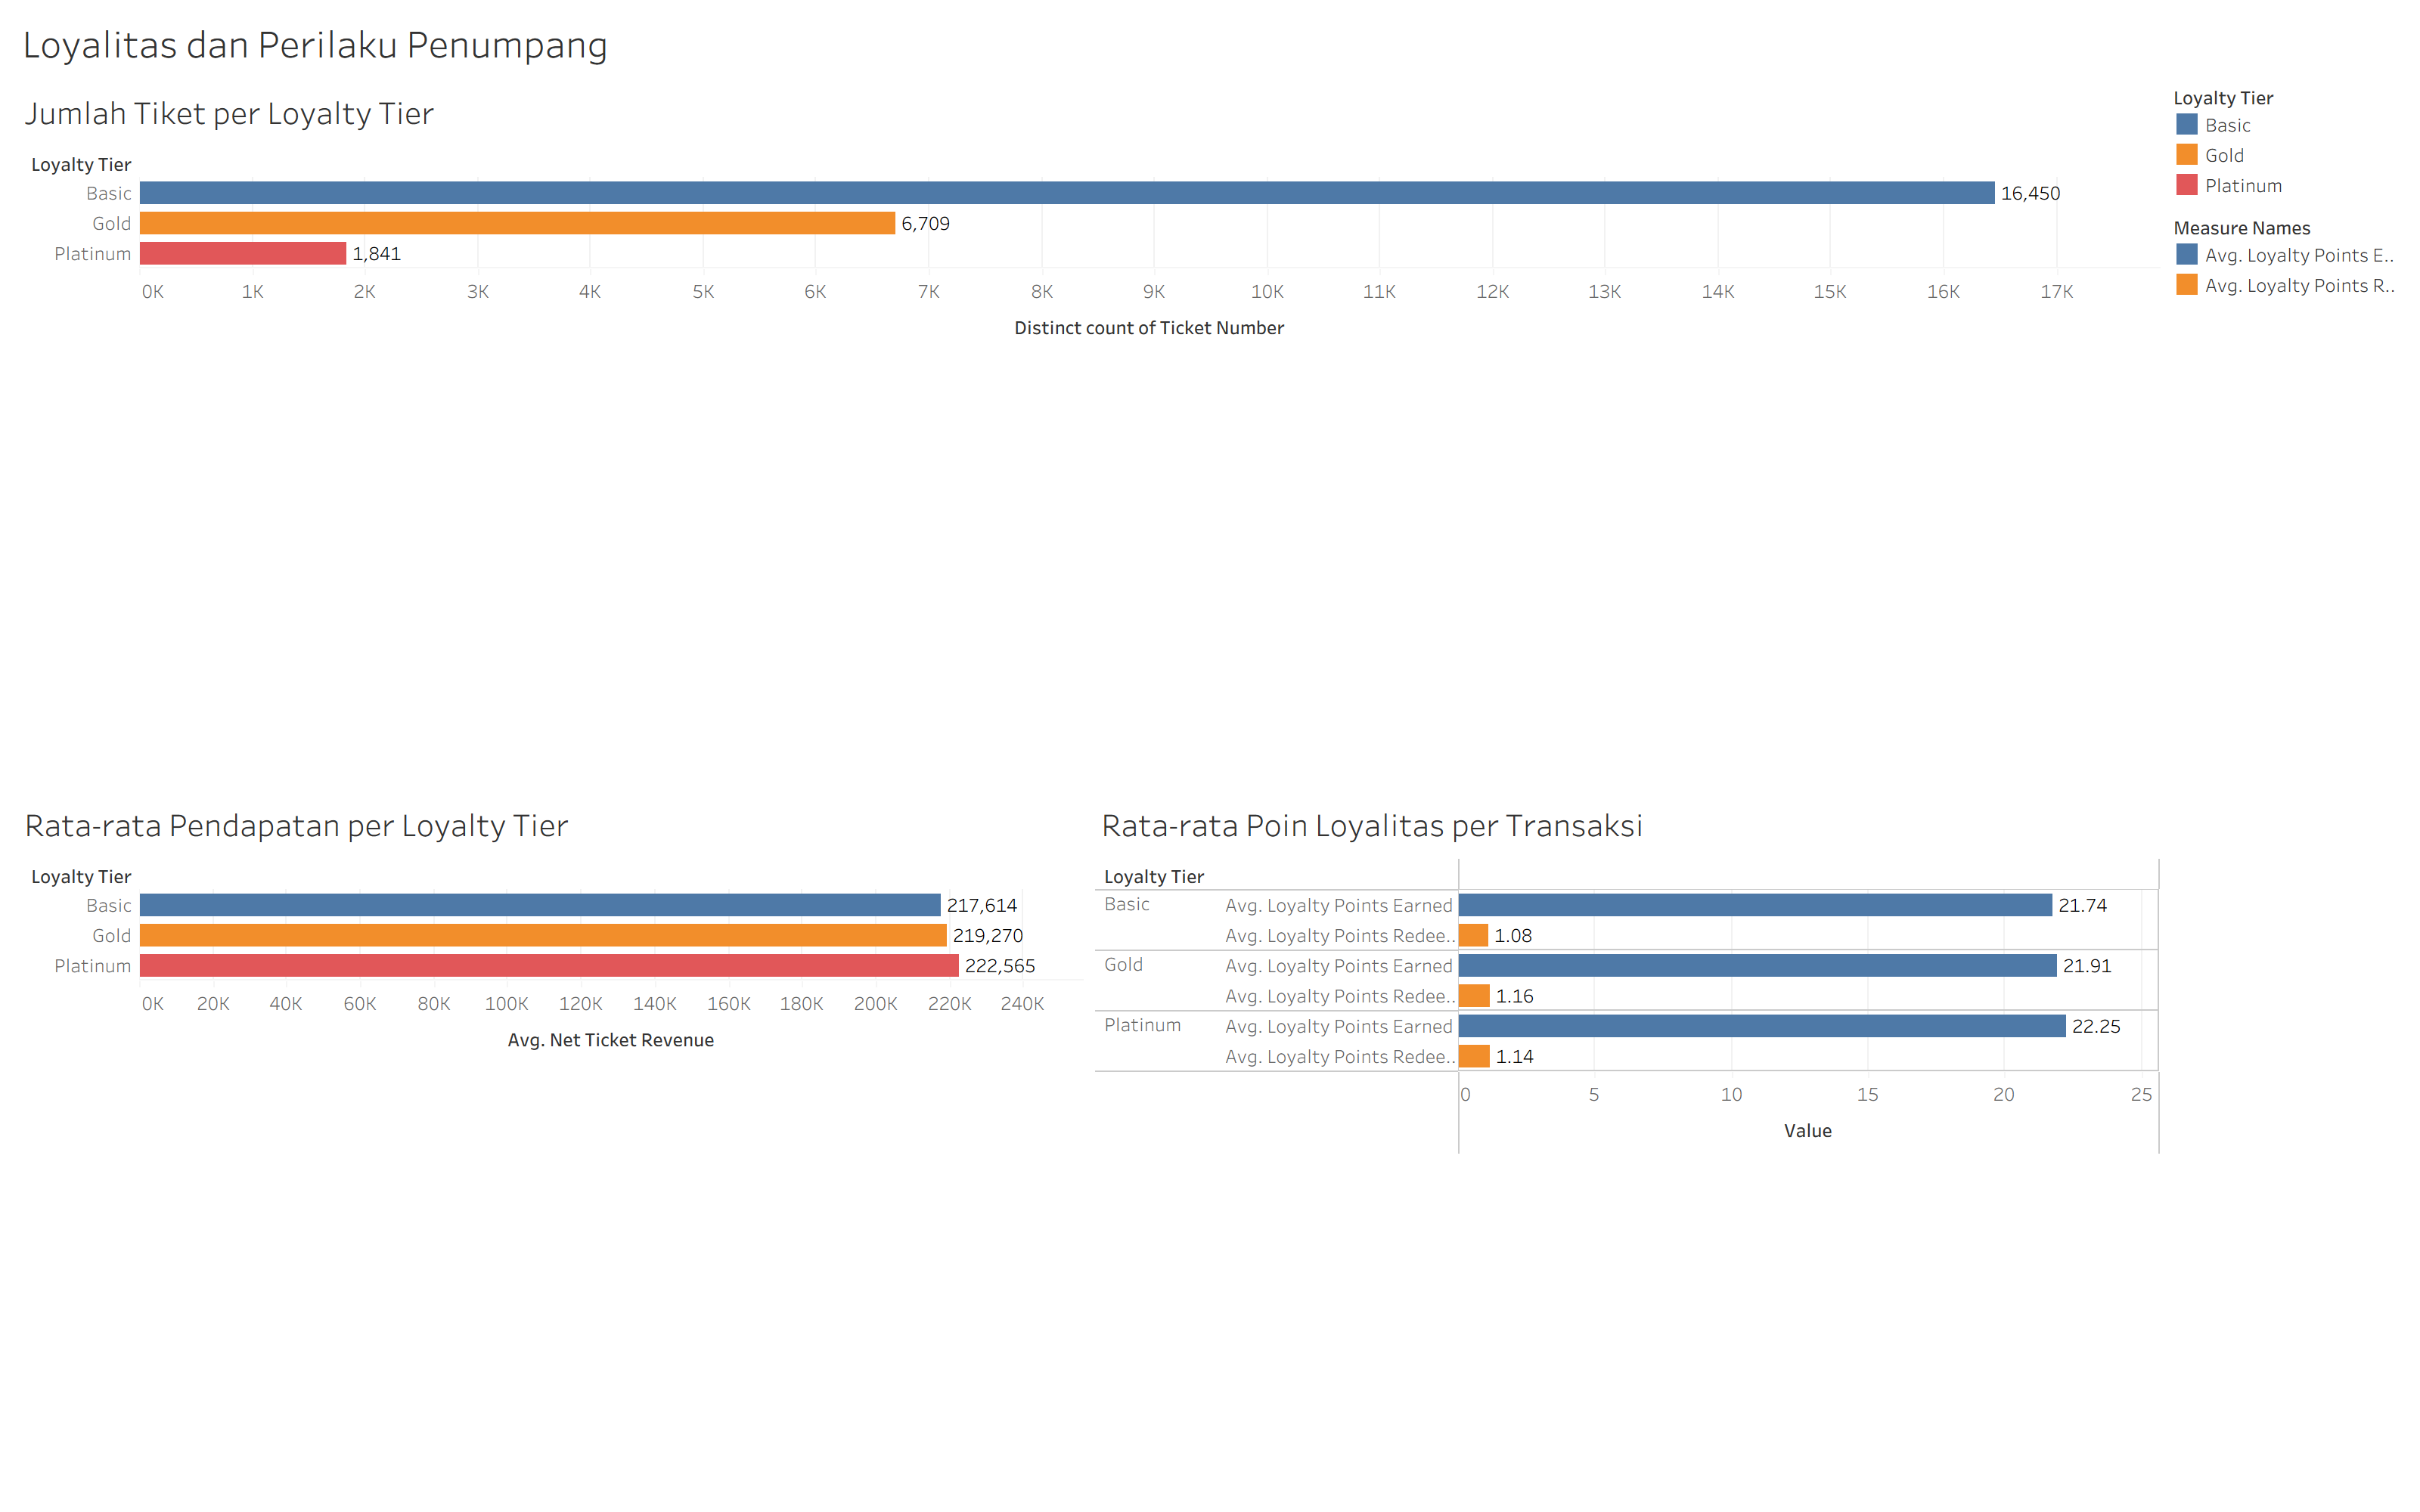
\includegraphics[width=\textwidth]{figures/dashboard-perilaku-loyalitas.png}
    \caption{Dashboard loyalitas dan perilaku penumpang}
    \label{fig:dashboard-perilaku-loyalitas}
\end{figure}

Gambar \ref{fig:dashboard-perilaku-loyalitas} menunjukkan bahwa tier Basic
mencatat 16.450 tiket, Gold 6.709 tiket, dan Platinum 1.841 tiket. Rata-rata
\texttt{net\_ticket\_revenue} menunjukkan pola yang berbeda: Platinum memiliki
nilai tertinggi sebesar Rp222.565, diikuti Gold Rp219.270 dan Basic Rp217.614.
Nilai ini mencakup pajak, sedangkan visual Python mengikuti gross revenue pada
query Bab 1.6 yang dihitung dari tarif setelah diskon sebelum pajak.

Rata-rata poin yang diperoleh berada pada kisaran 21,74--22,25 poin per transaksi,
sedangkan rata-rata poin yang ditukarkan berada pada kisaran 1,08--1,16 poin per
transaksi. Pada data sintetis ini, aktivitas memperoleh poin lebih dominan daripada
penggunaan poin.

\subsection{Dashboard Aktivitas Transaksi Loyalitas}

\begin{figure}[htbp]
    \centering
    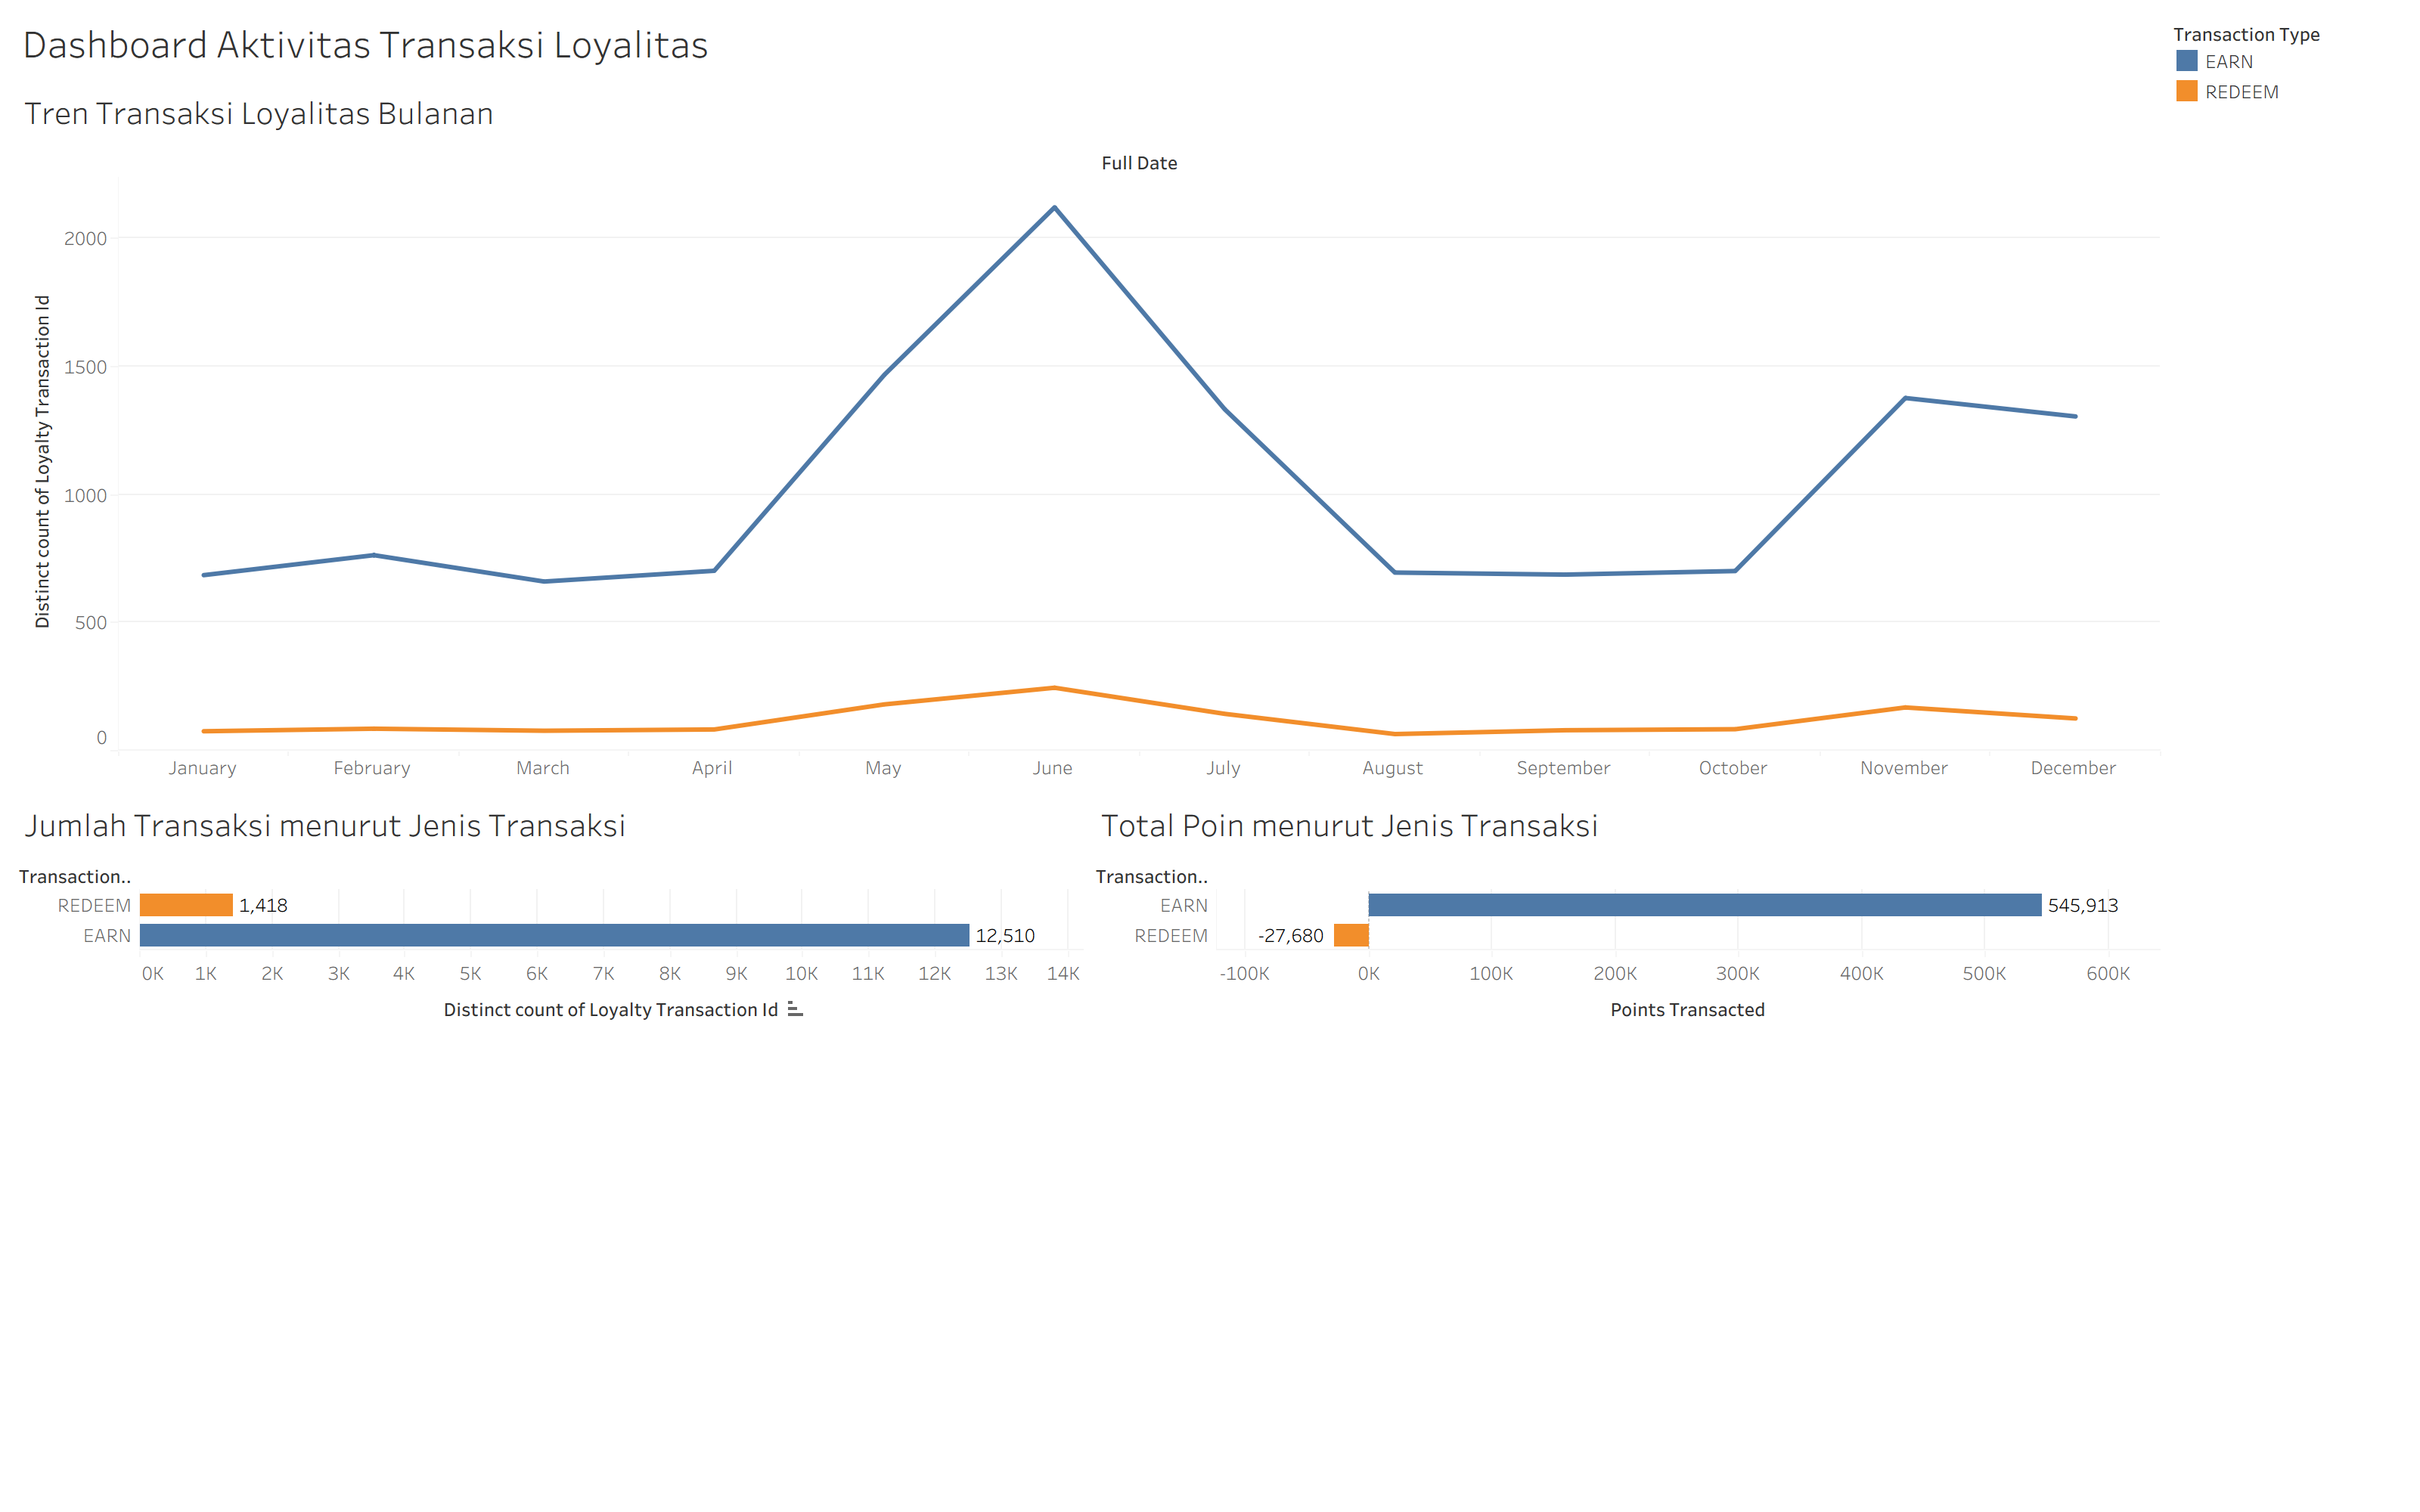
\includegraphics[width=\textwidth]{figures/dashboard-transaksi-loyalitas.png}
    \caption{Dashboard aktivitas transaksi loyalitas}
    \label{fig:dashboard-transaksi-loyalitas}
\end{figure}

Dashboard pada Gambar \ref{fig:dashboard-transaksi-loyalitas} menggunakan
\texttt{fct\_loyalty\_transaction}. Terdapat 12.510 transaksi \texttt{EARN} dan
1.418 transaksi \texttt{REDEEM}. Total poin yang diperoleh mencapai 545.913 poin,
sedangkan penukaran tercatat sebagai mutasi negatif sebesar 27.680 poin.

Aktivitas transaksi meningkat pada Juni serta kembali naik pada November dan
Desember. Pola tersebut konsisten dengan skenario peak season yang dimasukkan saat
pembangkitan data. Nilai negatif pada transaksi \texttt{REDEEM} dipertahankan agar
arah perubahan saldo dapat dibedakan dari perolehan poin.

\section{Pembahasan}

Ketiga dashboard menunjukkan bahwa fact table pada data mart dapat digunakan
sesuai proses bisnisnya. Dashboard operasional menghubungkan gangguan perjalanan
dengan dampak finansial, sedangkan dua dashboard loyalitas membedakan profil
penjualan tiket dari mutasi poin. Pemisahan ini menjaga agar metrik pada grain
tiket, penumpang-leg, dan transaksi poin tidak saling menggandakan nilai.

Dashboard Tableau menyediakan tooltip dan filter sesuai konteks visual. Grafik
batang menggunakan label angka agar perbandingan tidak hanya bergantung pada
warna. Workbook disimpan sebagai \texttt{visualisasi-bus-antarkota.twbx} sehingga
relationship, calculated field, worksheet, dashboard, dan sumber CSV dapat dibuka
kembali sebagai satu paket.

Data yang digunakan bersifat sintetis sehingga pola yang terlihat tidak dapat
digeneralisasi sebagai kondisi operator bus nyata. Missed connection rate yang
tinggi juga perlu dibaca bersama jumlah observasinya. Hubungan gangguan perjalanan
dengan repeat booking masih berupa asosiasi dan memerlukan analisis lebih lanjut
sebelum digunakan untuk menarik kesimpulan kausal.

\section{Kesimpulan}

Tableau dan Python-based tools telah menggunakan keluaran data mart yang sama.
Tiga dashboard Tableau mendukung analisis operasional, komersial, dan loyalitas,
sedangkan dashboard Python menyajikan lima visual yang mengikuti business
questions dan query verifikasi. Metrik yang menggunakan definisi sama menghasilkan
angka yang konsisten, sedangkan perbedaan gross dan net revenue dijelaskan sesuai
kolom yang digunakan.
